\documentclass[10pt]{article}
\usepackage{amsfonts}
\usepackage{amsmath}
\usepackage[font=small,labelfont=bf]{caption}
\usepackage{fancyhdr}
\usepackage[margin=1.0in]{geometry}
\usepackage{graphicx}
\usepackage{hyperref}
\usepackage{multicol}
\usepackage{textcomp}
\setlength{\columnsep}{0.5cm}
\setlength{\headheight}{24pt}
\setlength{\parindent}{15pt}
\pagestyle{fancy}
\fancyhf{}
\lhead{
	CSE 847: Machine Learning---Final Report \\
	Langford, Lingg, and Lucero
}
\rhead{March 24, 2017}
\cfoot{\thepage}
\begin{document}
	\title{
		CSE 847: Machine Learning---Final Report \\
		\textbf{An Exploration and Implementation of Automated Valuation Models to Learn and Predict the Value of Real Estate}
	}
	\author{
		\begin{tabular}{ccc}
			Mick Langford & Mike Lingg  & Jordi Lucero \\
			langfo37@msu.edu & linggmic@egr.msu.edu & luceroj2@msu.edu
		\end{tabular}
	}
	\date{March 24, 2017}
	\maketitle
	\begin{multicols}{2}
		\section{Problem Description}
		Automated Valuation Models (AVM) have become increasingly popular as the real estate market has embraced the World Wide Web as a source of accurate, up to the minute data.\textsuperscript{\cite{kaggleblog}} Banks have also shown great interest in using AVMs to help mitigate fraud by human appraisal.\textsuperscript{\cite{scotsman}} Our goal is to explore various machine learning techniques to implement an AVM and predict the true value of a house based on features commonly found on real estate listings. Our data will be drawn from the Nashville, TN housing market, using a dataset posted on Kaggle\textsuperscript{\cite{nashville_data}}.
		\par
		We will begin by exploring linear regression models that take into account physical attributes of each house and location. Further work will be performed exploring nonlinear models, such as deep learning with neural networks and decision trees, which can be compared and contrasted. Additional work may be performed to explore missing feature estimation.
		\section{Related Work}
		An obvious and popular example is Zillow's proprietary Zestimate\textsuperscript{\textregistered}. Zillow uses a closed source AVM that takes into account special features of the home, location, and market conditions. Zillow admits to using features such as physical attributes, tax assessments, and prior transactions. Zillow claims to have data on 110 million homes and estimates on approximately 100 million homes.\textsuperscript{\cite{zillow}}
		\par
		Relevant papers include the doctoral dissertation of Lowrance which explores and compares various linear models on housing data for the Los Angeles County.\textsuperscript{\cite{lowrance}} Park and Bae explore machine learning algorithms such as C4.5, RIPPER, Naive Bayesian, and AdaBoost.\textsuperscript{\cite{park}} Bin performed a study that estimates a hedonic price function using a semi-parametric regression.\textsuperscript{\cite{bin}} This may be particularly useful for real estate listings that are incomplete or for data that is entered erroneously. Bourassa et al. consider the spatial dependence of house prices, which is intuitively an important factor.\textsuperscript{\cite{bourassa1}\cite{bourassa2}} Kauko et al. research neural network models to help investigate segmentation in the housing market of Helsinki, Finland.\textsuperscript{\cite{kauko}} Azadeh et al. present an algorithm based on fuzzy linear regression and a fuzzy cognitive map to handle uncertainty in the housing market and improve the analysis of housing price fluctuations.\textsuperscript{\cite{azadeh}} Fan et al. introduce a decision tree approach for modeling and predicting house prices.\textsuperscript{\cite{fan}}
		\section{Project Data}
		For this project we are working with multiple data sources pulled from real housing sales data.
		\par
		\textbf{Nashville Housing Data} The Nashville housing data set is a list of home sales in the Nashville, Tennessee area, provided by Kaggle\textsuperscript{\cite{nashville_data}}. This data set includes 29 fields of data for 56635 entries. However, nearly half of the entries have gaps in information, which will have to be accounted for. We further augmented this data set by using an geocoding service provided by the United State Census Bureau to add the zip code, latitude, and longitude for entries where a match could be found.
		\par
		\textbf{King County Housing Data} The King County housing data set is a list of home sales in the King County, Washington area, provided by Kaggle\textsuperscript{\cite{kc_data}}. This data set includes 20 fields of data for 21614 entries, with none of the entries missing any data.
		\par
		\textbf{Advanced Regression Techniques Data} The Advanced Regression Techniques data is a list of home sales, provided by Kaggle. This data includes 79 features of housing data for 1460 homes. The data has no gaps, except for some N/A data.
		\par
		\textbf{Grand Rapids Data} The Grand Rapids data is a list of home sales in the Grand Rapids area, provided by the real estate listing service Redfin. This data includes 16 fields for 9646 entries. The data set also has gaps in information for about half of the entries.
		\par
		The different data sets provide a variety of input to test machine learning techniques against. Data with more features should provide more accurate results, if the additional features provide useful information for the prediction.
		\section{Preprocessing Data}
		For pre-processing the data, we will be normalizing the data set, by dividing each feature value by the difference between that feature's maximum and minimum values. Another problem being considered is how to properly manage fields containing categorical values. Our approach will be to treat a field with \(n\) categories as \(n\) binary features, indicating whether that entry is of the associated category or not. Finally we provide the ability to fill in holes in the input data using the feature mean, closest value, by way of Euclidean distance, or closest mean.
                \par
		{\centering
        	\captionsetup{type=table}
			\begin{tabular}{r|c}
				& \small{Preprocessing Results} \\
				\hline
				\small{No Preprocessing} & \small{2.6e-3} \\
				\hline
				\small{Value Normalizing} & \small{2.3e-3} \\
				\hline
				\small{Normalize and Binary Features} & \small{2.0e-3} \\
				\hline
			\end{tabular}
			\captionof{table}{Linear regression preprocesssing results.}
			\label{table:linr_preprocessing}        
		\setlength{\parindent}{15pt} }
                \par
                Table \ref{table:logr_preprocessing} shows the results of data preprocessing with a simple closed form linear regression, using the Advanced Regression Techniques Data. Note, the first row with no preprocessing does normalize the sale prices so the mean squared error can be compared between the results. The first row shows that without normalizing the data, there is very little accuracy in the predictions. Simply normalizing all of the data provides a significant increase in accuracy of the predictions. Finally, by splitting category fields into binary features, the error is improved by more than 15\%.
                \par
		{\centering
        	\captionsetup{type=table}
			\begin{tabular}{r|c}
				& \small{Hole Filling} \\
				\hline
				\small{None} & \small{NaN} \\
				\hline
				\small{Mean} & \small{1.6e-3} \\
				\hline
				\small{Closest Value} & \small{1.2e-3} \\
				\hline
				\small{Closest Mean} & \small{1.1e-3} \\
				\hline
			\end{tabular}
			\captionof{table}{Linear regression preprocesssing hole filling results.}
			\label{table:linr_hole_fill}        
		\setlength{\parindent}{15pt} }
                \par
                Additionally we look at the best method of filling in holes in the input data. The Advanced Regression Techniques Data has no holes so we look at the Grand Rapids Data from Redfin for hole filling. Table \ref{table:logr_hole_fill} shows that with no holes filled, the basic closed form linear regression cannot be solved with Matlab. From the remaining methods, Closest Mean provides the most accurate predictions.
 		\section{Models}
		Figure \ref{fig:ganttchart} shows our initial project milestones and timeline to completing them.
	\end{multicols}
	\begin{figure*}[h]
	    \centering
	    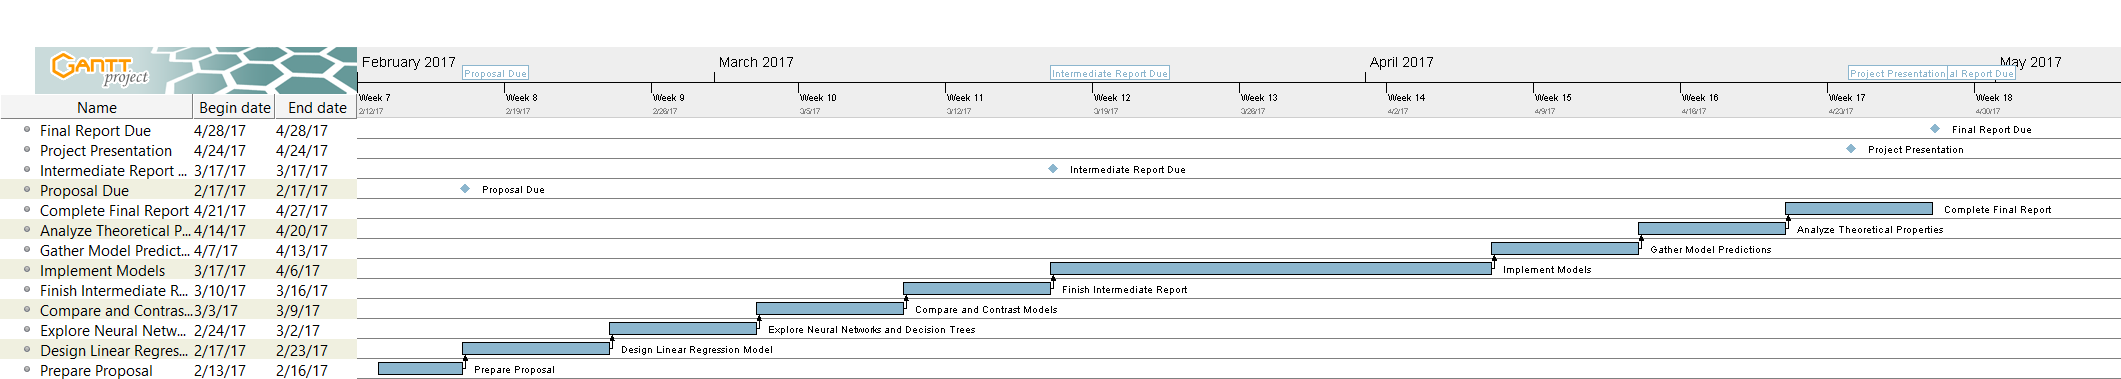
\includegraphics[width=\textwidth]{Schedule/ProjectSchedule.png}
	    \caption{Gantt Chart showing  our project milestones and expected completion dates.}
	    \label{fig:ganttchart}
	\end{figure*}
	\begin{multicols}{2}
		\subsection{Linear Regression}
			For linear regression we are using a closed form ridge regression. We tested standard and stochastic gradient descent but these methods did not produce a significant improvement in processing time for the data we are using and do not improve on the prediction error.
		\par
			For the ridge regression regularization value we developed a simple automated approach to identify the ideal regularization value. We start with a test regularization value of 1 and perform five fold cross validation on the training data to determine the mean square error with this test value. Then we adjust the test value by 10 in the positive direction, in this case moving from 1 to 11, and repeat the cross validation. If the error decreases, we continue to adjust the test value in the same way. If the error increases, we reverse the sign of the test value adjustment and divide it by 10. This is similar to a simplistic gradient descent, but when we overshoot the minimum we reverse direction and lower the step size.  This continues until the error between two cross validations matches within 1e-7.
		\par
		\begin{center}
                  \captionsetup{type=figure}
			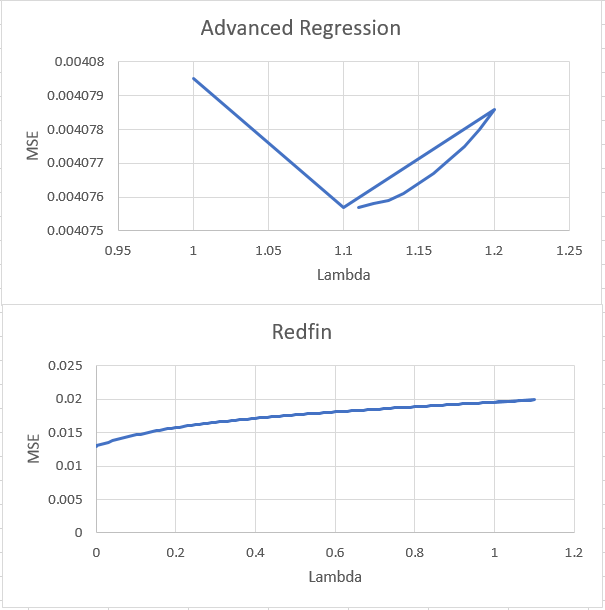
\includegraphics[scale=0.35]{Images/LinearRegressionCrossTrain} \\
			\captionof{figure}{Linear regression cross training.}
			\label{fig:linr_cross_train}
		\end{center}
		\par
                Figure \ref{fig:linr_cross_train} shows the results of our cross training method on the Nashville, Advanced Regression and Redfin data sets.  The Nashville set has a high ideal regularization value, likely due to a few very high value homes in the data set, and the training simply continues to increase the regularization value until the minimum error is found.  The advanced regression data set has reduced error from regularization value of 1 to 11 but then the error increases from 11 to 21.  Then the advanced regression moves back down from 21 at a lower rate until the minimum value is found around 4.  This shows a place where the algorithm works but could be made more efficient.  Finally the Redfin data starts at a regularization value of 1 but sees an increase of error at 11 so decreases until it finds the ideal value was in fact near 1.
		\par
                
 		\subsection{Classification}
			We are also approaching this problem as a classification problem for our linear regression and neural network models. The range of sale prices for the entire data set will be partitioned into \(k\) classes, each class can include the same range of values, or be variable in size to accommodate ranges with similar input data. The classification solutions will then be fitted to a training data set, and finally predict each entry in the test data set by fitting it into one of the \(k\) classes.
		\subsection{Logistic Regression}
			During initial logistic regression development, we have used two different approaches to perform classification.
		\par
			The first approach attempt to classify which of the k class ranges the house most likely falls in based on input data. This model is composed of a matrix of independent regression models. It is trained for each input data point by setting the Y value corresponding with the class the house value falls under to 1 and all others to 0. The current training method uses stochastic gradient descent with a reducing step size. Once trained, the logistic regression class with the most confident result for the given input data is the one under which we classify a house.
		\par
	 		The second approach also uses a matrix of independent regression models but instead the results classify if the house is worth more than the lower value of the class k of each model. The training method only differes from the first approach by setting the Y value corresponding with the class equal to 1 if the value of the current house is higher than the lower value of the class. Then classification is performed by summing up the range represented by each class with a confidence higher than 0.5.
		\par
 			Table \ref{table:logr_performance} shows that the second approach for logistic regression, determining if the house is worth more than each class, works better than the first approach, determining which class the house would fall under. The second approach also produces a result much faster than the first approach. However, both approaches have a bit higher MSE when compared with the ideal linear regression model. At the same time, the logistic regression models appear to do a better job of classifying prices at the higher price range, where linear regression performed more poorly.
		\par
        	\captionsetup{type=table}
			\begin{tabular}{r|c}
				& \small{Mean Squared Error} \\
				\hline
				\small{Linear Regression Mode} & \small{1.3e+09} \\
				\hline
				\small{Logistic Regression Model 2} & \small{1.4e+09} \\
				\hline
				\small{Logistic Regression Model 1} & \small{2.9e+09} \\
				\hline
			\end{tabular}
			\captionof{table}{Observed performance from logistic regression model.}
			\label{table:logr_performance}        
			\setlength{\parindent}{15pt}
		\par
 			Moving forward in the project we are looking at attempting to combine the strengths of the two approaches. To do this we intend to use logistic regression to identify ranges where the test data can be represented by similar models. Then logistic regression can be used to model each section without being influenced by data in the other sections. However, a simpler solution might simply be to transform the training data to use the logarithm of the house prices.
		\subsection{Decision Tree}
		\par
		For our Decision Tree approach, we used a Classification Decision Tree and a Regression Decision Tree. For the Classification Tree, since the data was not already classified, it was split into \(k\) equally sized classes where each class represents a range of prices. The average value for every feature column is also calculated and used to subsitute for any missing data points in the observations. A classification model was built for the KC data set, Redfin data set, and Nashville data set. For each data set, initially a classification tree model was built using crossfold validation with 10 folds using 90\% of the data for training. This model used the default parameters for tree size, which are maximum number of splits of n-1, minimum leaf size of 1, and minimum parent size of 1. 
		\par		
Another classification model was built by using 10 fold cross validation and generating trees for many possible parameters and choosing the model that provides the best training MSE, again using 90\% of the data for training. The results comparing these two models and their training and testing MSEs for the Nashville data set is shown in Table \ref{table:ctree_performance} below. The MSE indicates the averae squared distance between the predicted class and the actual class, where the classes are represented by a range of integers from 1 to \(k\). In the results below, the number of classes that are being classified is 8.
		\par
		\captionsetup{type=table}
			\begin{tabular}{r|c}
				& \small{Mean Squared Error} \\
				\hline
				\small{CTree Train Error} & \small{0.2890} \\
				\hline
				\small{CTree Test Error} & \small{0.5247} \\
				\hline
				\small{Optimized CTree Train Error} & \small{0.5052} \\
				\hline
				\small{Optimized CTree Test Error} & \small{0.4350} \\
				\hline
			\end{tabular}
			\captionof{table}{Observed performance from Classification Tree models.}
			\label{table:ctree_performance}        
			\setlength{\parindent}{15pt}
		\par
		For the Classification Tree, the optimized parameters result in much higher testing error, but also a much better testing error. This seems to indicate that default parameters with crossfold validation result in slight overfitting compared to crossfold validation with the optimized parameters.
		\par
		Regression Tree models were generated following a similar pattern, creating one 10 fold cross validation Regression Tree model for each data set using default parameters and creating another Regression Tree model by varying the tree parameters to find the best MSE training error. Table \ref{table:rtree_performance} below shows a table of the MSE results for the Regression Tree approach on the Nashville data set. 
		\par
		\captionsetup{type=table}
			\begin{tabular}{r|c}
				& \small{Mean Squared Error} \\
				\hline
				\small{RTree Train Error} & \small{5.4526e+10} \\
				\hline
				\small{RTree Test Error} & \small{6.8929e+10} \\
				\hline
				\small{Optimized RTree Train Error} & \small{5.2162e+10} \\
				\hline
				\small{Optimized RTree Test Error} & \small{6.5855e+10} \\
				\hline
			\end{tabular}
			\captionof{table}{Observed performance from Regression Tree models.}
			\label{table:rtree_performance}        
			\setlength{\parindent}{15pt}
		\par
		The Regression models perform similarly, with slightly better results using the optimized parameters for the regression tree compared to the default parameters. Our goal for the Decision Tree approach is to take the best approach and vary the feature selection to create a Random Tree Forest. Then use proximity trees to better estimate any missing values.
		\subsection{Neural Network}
		\par
		Our initial approach for implementing a neural network learning model is to use a simple feed-forward network with three hidden fully-connected layers. Each data point will have \(d\) features extracted from the data. Each feature in the input will have its value sent as input to each neuron in the first layer of the network, where each neuron has its own associated weight and activation function. Each neuron's output from the first layer will be sent as input to each neuron in the second layer, which will also have its own weight values and activation function. Finally, the output from each neuron in the second layer will be sent as input to each neuron in the third layer, again having its own weights and activation function. The final hidden layer will have \(k\) outputs, representing which class the data point falls into.
		\par
		Our current method is to use a sigmoid function as the activation function for each layer, with \(k\) neurons in the third layer, \(2k\) neurons in the second layer, and \(4k\) neurons in the third layer. Further experimentation is being conducted with varying sizes and architectures.
		\begin{center}
            \captionsetup{type=figure}
			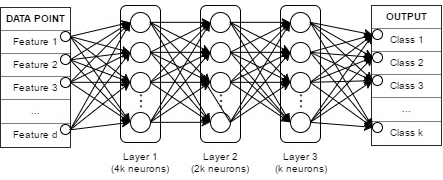
\includegraphics[scale=0.5]{NeuralNet/Network} \\
			\captionof{figure}{Architecture of our network.}
			\label{fig:nn_10_class_results}
		\end{center}
		The input data is randomly shuffled and split into training and testing data sets, with a ratio of \(9:1\). The model is trained for 50 epochs, using an Adaptive Gradient Descent (Adagrad) algorithm to fit and optimize weights throughout the model, with an initial learning rate \(\eta = 0.1\). Techniques are being considered that will decay the learning rate with relation to the loss calculated for each epoch.
		\par
		Displayed in Table \ref{table:nn_performance} and Figures \ref{fig:fig_nn_results_5} and \ref{fig:fig_nn_results_10} are the results of running the data sets through the current prototype network. Two different trials were run on each data set, with the first trial learning and predicting against 5 classes of target values, and the second trial against 10 classes of target values. Each target class represents an equally sized partition of the data's target values. Predictions of a target class indicate that the given data point's sale price will fall within the boundaries that define that class's partition.
		\begin{center}
            \captionsetup{type=table}
			\begin{tabular}{r||c|c||c|c}
				& \multicolumn{2}{c||}{\small{5 classes}} & \multicolumn{2}{c}{\small{10 classes}} \\
				\hline 
				& \small{Train} & \small{Test} &  \small{Train} & \small{Test} \\
				\hline
				\small{Nashville} & \small{61.53\%} & \small{60.41\%} & \small{39.80\%} & \small{38.71\%} \\
				\hline
				\small{King County} & \small{51.92\%} & \small{51.92\%} & \small{30.90\%} & \small{29.94\%} \\
				\hline
				\small{Grand Rapids} & \small{57.05\%} & \small{56.34\%} & \small{33.74\%} & \small{32.75\%} \\
				\hline
			\end{tabular}
			\captionof{table}{Observed performance from neural network.}
			\label{table:nn_performance}
		\end{center}
		\begin{center}
            \captionsetup{type=figure}
			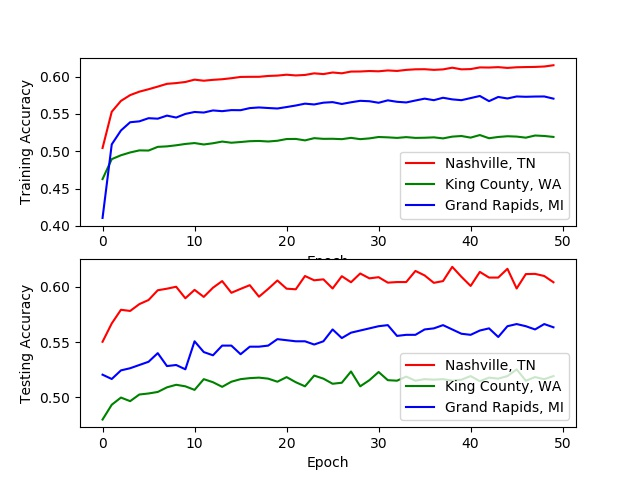
\includegraphics[scale=0.38]{NeuralNet/nn_5_class_results} \\
			\captionof{figure}{Results for classifying into 5 classes.}
			\label{fig:fig_nn_results_5}
		\end{center}
		\begin{center}
            \captionsetup{type=figure}
			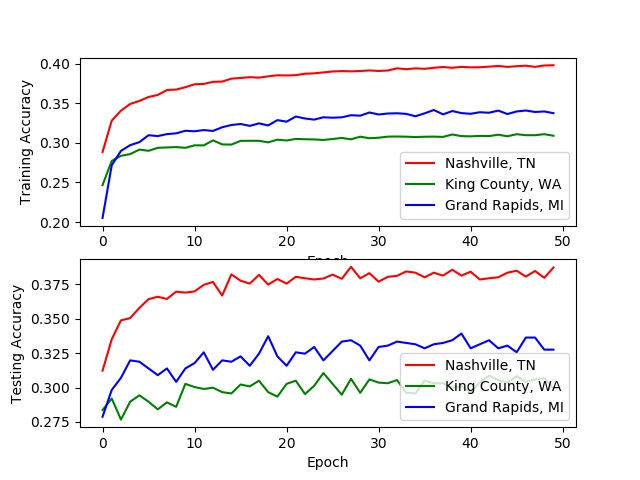
\includegraphics[scale=0.38]{NeuralNet/nn_10_class_results} \\
			\captionof{figure}{Results for classifying into 10 classes.}
			\label{fig:fig_nn_results_10}
		\end{center}
		The results show that the network performs better when classifying data points into a smaller number of target classes. Our goal from this point forward is to attempt to improve accuracy by investigating further improvements on preprocessing the input data, experimenting with different hyper-parameters for the network, and experimenting with varying network architectures. When accuracy improves, the goal with then be to increase the number of target classes in order to provide a more valuable estimation of the sales price of any given data point.
		\begin{thebibliography}{13}
			\bibitem{nashville_data}
			\textit{Nashville Housing Data: Home value data for the booming Nashville Market}
			Retrieved from \\ \small{\url{https://www.kaggle.com/tmthyjames/nashville-housing-data/}}
			
			\bibitem{kc_data}
			\textit{House Sales in King County, USA: Predict house price using regression}
			Retrieved from \\ \small{\url{https://www.kaggle.com/harlfoxem/housesalesprediction}}	
			
			\bibitem{kaggleblog}
			\textit{Data-driven property valuations: the real deal?}
			Retrieved from \\ \small{\url{http://blog.kaggle.com/2010/06/21/data-inc-are-avms-soothsayers-or-the-real-deal/}}
			
			\bibitem{scotsman}
			Schroeder, Steve.
			\textit{Fighting Fraud: A combination of collateral assessment and AVMs can maximize mortgage-fraud management}
			Retrieved from \\ \small{\url{http://www.scotsmanguide.com/Residential/Articles/2005/10/Fighting-Fraud/}}
			
			\bibitem{zillow}
			\textit{What is a Zestimate? Zillow's Home Value Forecast.}
			Retrieved from \\
			\small{\url{http://www.zillow.com/zestimate/}}
			
			\bibitem{lowrance}
			Lowrance, R. E. (2015).
			\textit{Predicting the Market Value of Single-Family Residential Real Estate}
			(Doctoral Dissertation). New York University. Retrieved from \small{\url{http://gradworks.umi.com/36/85/3685886.html}}
			
			\bibitem{park}
			Park, B., \& Bae, J. K. (2015).
			\textit{Using machine learning algorithms for housing price prediction: The case of Fairfax County, Virginia housing data.}
			Expert Systems with Applications, 42(6), 2928-2934. doi:10.1016/j.eswa.2014.11.040
			
			\bibitem{bin} 
			Bin, O. (2004).
			\textit{A prediction comparison of housing sales prices by parametric versus semi-parametric regressions.}
			Journal of Housing Economics, 13(1), 68-84. doi:10.1016/j.jhe.2004.01.001
			
			\bibitem{bourassa1} 
			Bourassa, S. C., Cantoni, E., \& Hoesli, M. (2010). 
			\textit{Predicting House Prices with Spatial Dependence: Impacts of Alternative Submarket Definitions.}
			SSRN Electronic Journal. doi:10.2139/ssrn.1090147
			
			\bibitem{bourassa2}
			Bourassa, S. C., Cantoni, E., \& Hoesli, M. (2007).
			\textit{Spatial Dependence, Housing Submarkets, and House Prices.}
			SSRN Electronic Journal. doi:10.2139/ssrn.771867
			
			\bibitem{kauko}
			Kauko, T., Hooimeijer, P., \& Hakfoort, J. (2002).
			\textit{Capturing Housing Market Segmentation: An Alternative Approach based on Neural Network Modelling.}
			Housing Studies, 17(6), 875-894. doi:10.1080/02673030215999
			
			\bibitem{azadeh} 
			Azadeh, A., Ziaei, B., \& Moghaddam, M. (2012).
			\textit{A hybrid fuzzy regression-fuzzy cognitive map algorithm for forecasting and optimization of housing market fluctuations.}
			Expert Systems with Applications, 39(1), 298-315. doi:10.1016/j.eswa.2011.07.020
			
			\bibitem{fan}
			Fan, G., Ong, S. E., \& Koh, H. C. (2006).
			\textit{Determinants of House Price: A Decision Tree Approach.}
			Urban Studies, 43(12), 2301-2315. doi:10.1080/00420980600990928
		\end{thebibliography}
	\end{multicols}
\end{document}
